\documentclass[a4paper, 11pt, titlepage]{article}
\usepackage{graphicx}
\usepackage{pdfpages}
\usepackage{fancybox}
\usepackage[francais]{babel}
\usepackage[utf8]{inputenc}
% \usepackage[T1]{fontenc}
\usepackage{amsmath,amsfonts,amssymb}
\usepackage{fancyhdr}
\usepackage{stackrel}
\usepackage{babel,indentfirst}
\usepackage{xspace}
\usepackage{url}
\usepackage{titling}
\usepackage{listings}
\usepackage{color}
\usepackage{array}
\usepackage{hyperref}
\usepackage{makecell}
\usepackage{tikz}
\usepackage{float}

%\setlength{\parindent}{0pt}
\setlength{\parskip}{1ex}
\setlength{\textwidth}{17cm}
\setlength{\textheight}{24cm}
\setlength{\oddsidemargin}{-.7cm}
\setlength{\evensidemargin}{-.7cm}
\setlength{\topmargin}{-.5in}


\lstset{
  sensitive=f,
  morestring=[d]",
  showstringspaces=false,
  basicstyle=\small\ttfamily,
  keywordstyle=\bf\small,
  commentstyle=\itshape,
  stringstyle=\sf,
  extendedchars=true,
  columns=[c]fixed
}



\predate{
\begin{center}
}
\postdate{
\\
\vspace{1.5cm}

\includegraphics[scale=0.7]{imag.png}
\end{center}}


\title {{ {\huge Compte rendu du projet ACVL / Web }} }

\author{\Large Equipe 14 \\
\\
    {\sc Aboubacar}~Salim\\
    {\sc Demets}~Jules-Eugène\\
    {\sc Gouttefarde}~Léo\\
    {\sc Rey}~Simon
}

\date{Jeudi 14 Avril 2016}

\lhead{Projet ACVL / Web}
\rhead{Compte rendu}

\begin{document}
\pagestyle{fancy}
\maketitle

\setcounter{tocdepth}{2}

\tableofcontents
\newpage

% \begin{center}
% \section* {Introduction }
% \end{center}


% (a) Document d’analyse :
% — acteurs, diagramme de cas d’utilisations et description de ces cas d’utilisations, illustrées par des diagrammes de séquence système pertinents.
% — diagramme de classes d’analyse.

\section {Analyse}

Le sujet présente une application de gestion de jeux de rôle pour une association.

\subsection{Acteurs}

Seuls deux types d'acteurs peuvent intervenir dans cette application : les joueurs eux mêmes (c'est-à-dire les rôlistes) ainsi que les meneurs de jeu, qui dirigent les parties.

\subsection{Cas d'utilisation}

\subsubsection{Description des différents cas d'utilisation}

Voici les différents cas d'utilisation de l'application issus du cahier des charges, ils sont résumés dans un diagramme à la fin de cette section.

\begin{enumerate}
    \item Un joueur peut consulter la biographie d'un personnage 
        \begin{enumerate}
            \item  S'il possède le personnage il peut voir les paragraphes privés de la biographie.
            \item De même le meneur de jeu d'un personnage peut voir les paragraphes privés du dit personnage.
        \end{enumerate}
    \item Un joueur peut révéler des paragraphes secrets des biographies des personnage qu'il possède 
    \begin{enumerate}
        \item  L'application doit demander une validation pour cette action.            
    \end{enumerate}
      \item Un joueur peut créer un personnage 
      \begin{enumerate}
        \item  Le joueur doit alors indiquer : nom, date de naissance, profession ainsi qu'une biographie initiale
        \item Le joueur peut soumettre le personnage ainsi créé à un meneur de jeu
        \item Le meneur de jeu peut accepter le personnage, il peut lire la biographie (y compris les parties secrètes).
      \end{enumerate}
      \item Le meneur de jeu, ou un joueur, peut ajouter des épisodes à la biographie d'un de ses personnages 
      \begin{enumerate}
        \item Il en spécifie la date
        \item Il peut spécifier une aventure à laquelle est rattaché cet épisode. 
        \item  Il peut sauvegarder l'épisode en cours de rédaction.
        \item Il peut reprendre l'édition.
        \item Il peut supprimer l'épisode en cours d'édition
        \item Il peut le valider
        \item Une fois validé par le joueur et le meneur de jeu l'épisode devient définitif : il ne peut plus être modifier.
      \end{enumerate}
      \textit{De ce fait il est impossible de valider un épisode si le personnage n'a pas de meneur de jeu associé.}
    \item Un joueur peut proposer d'organiser une partie
    \begin{enumerate}
        \item  Il indique alors : titre, univers dans lequel se déroule la partie, situation initiale date et lieu
        \item La proposition est alors visible par tous.
        \item Le meneur de jeu peut ajouter ou enlever des personnages, ceux-ci doivent être du même univers que la partie et il doit être le meneur de jeu des personnages
        \item La proposition peut être supprimée
    \end{enumerate}
    \item Le meneur de jeu peut saisir un résumé des événements et indiquer la fin de la partie
    \begin{enumerate}
        \item Les éléments relatifs à la partie ne sont dés lors plus modifiables.
        \item La partie devient une aventure pouvant apparaitre dans la biographie des personnages.

    \end{enumerate}
    \item Un joueur peut modifier la profession de son personnage
    \begin{enumerate}
        \item Il indique la nouvelle profession du personnage
    \end{enumerate}
    \item Un joueur peut céder son personnage
    \begin{enumerate}
        \item Il indique le joueur bénéficiaire
    \end{enumerate}
    \item Un joueur peut changer le meneur de jeu d'un de ses personnages
    \begin{enumerate}
        \item Le nouveau meneur de jeu doit accepter.
        \item Ce transfert ne peut avoir lieu que si le personnage n'est pas impliqué dans une partie en cours.
    \end{enumerate}
    \end{enumerate}

\subsubsection{Diagramme des cas d'utilisation}

\begin{center}
% \begin{figure}[ht!]
    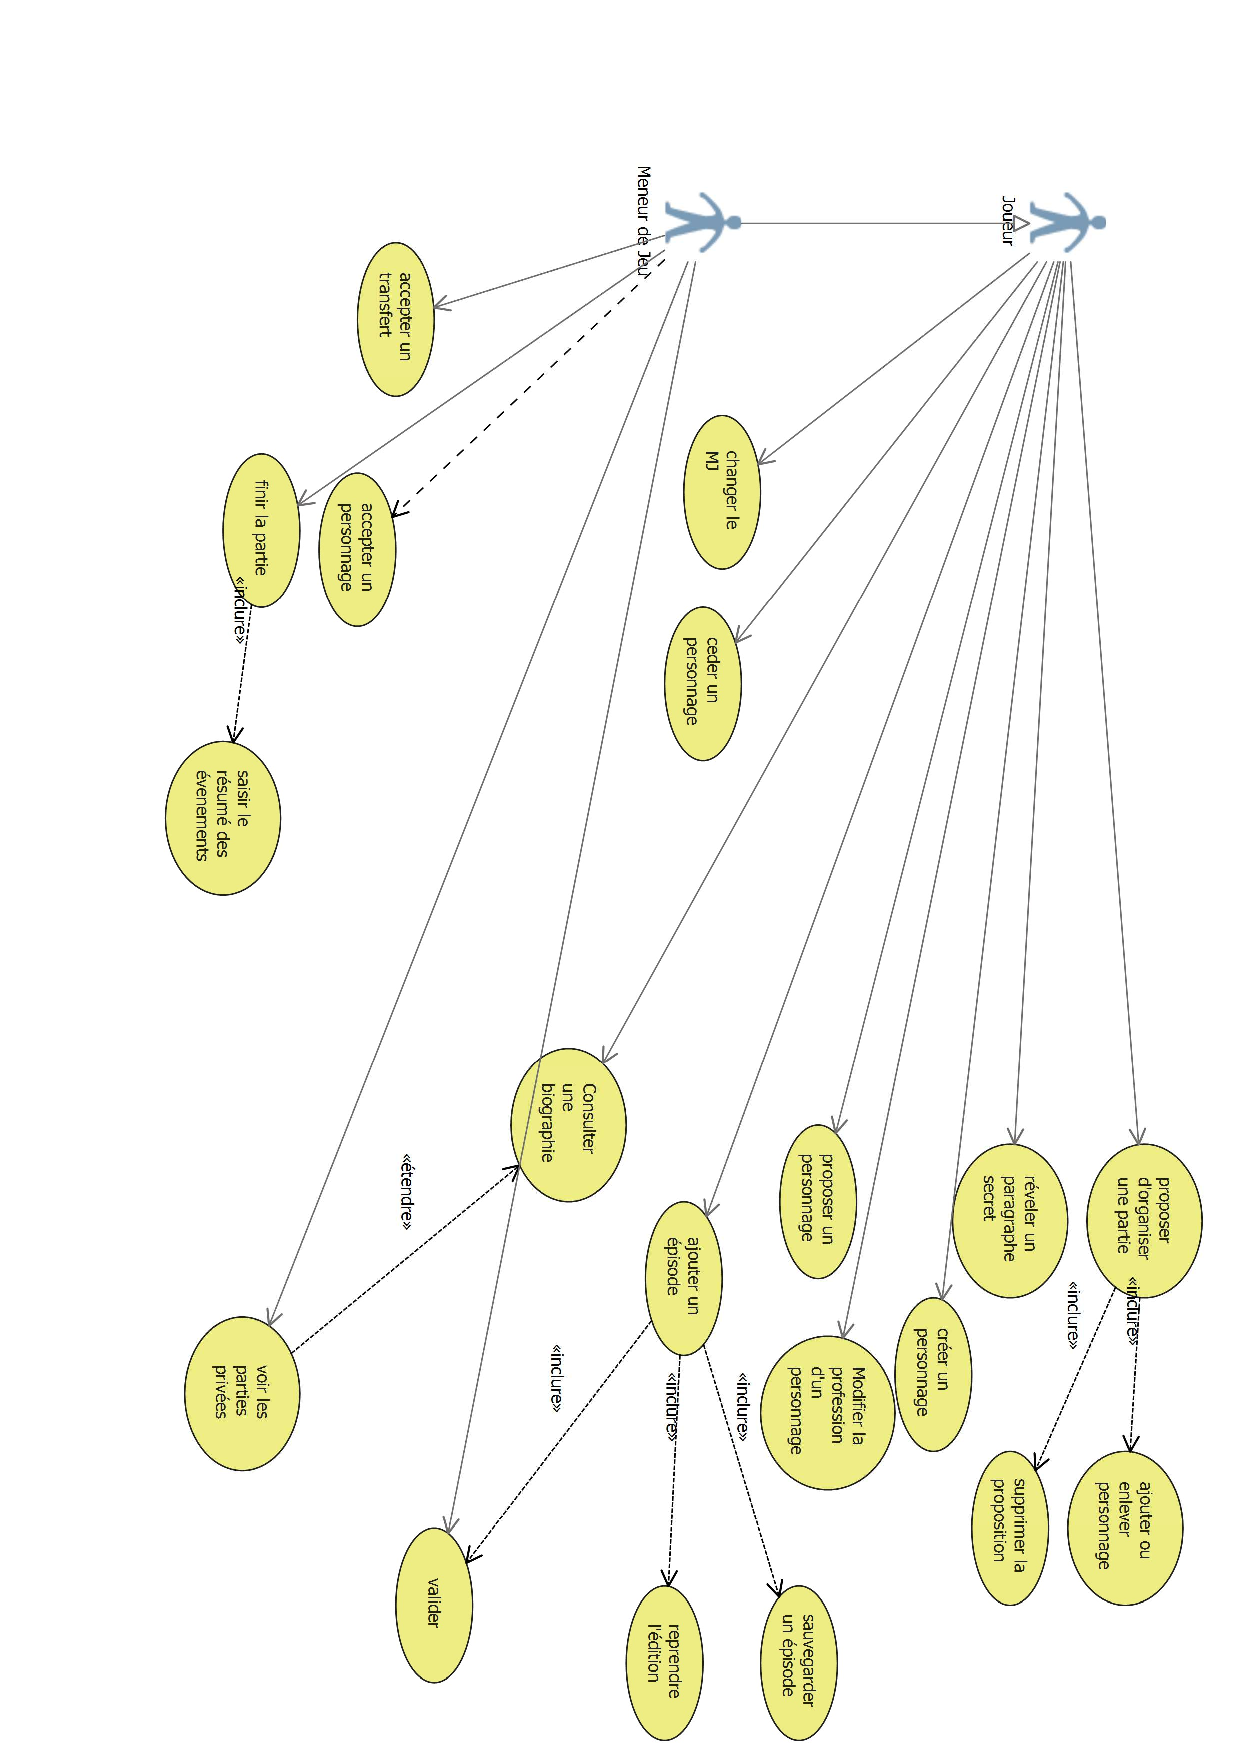
\includegraphics[scale=0.7]{analyse/cadutilisation}
% \caption{Diagramme des cas d'utilisation}
% \end{figure}
\end{center}


\newpage
\subsection{Diagrammes de séquence d'analyse}

\subsubsection{Révéler un paragraphe}

\begin{center}
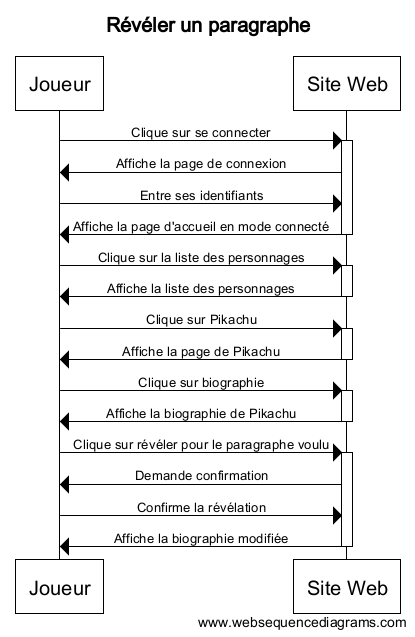
\includegraphics[scale=0.7]{sequence/RevelerParagAnalyse.png}
\end{center}

\subsubsection{Ajouter un épisode}

\begin{center}
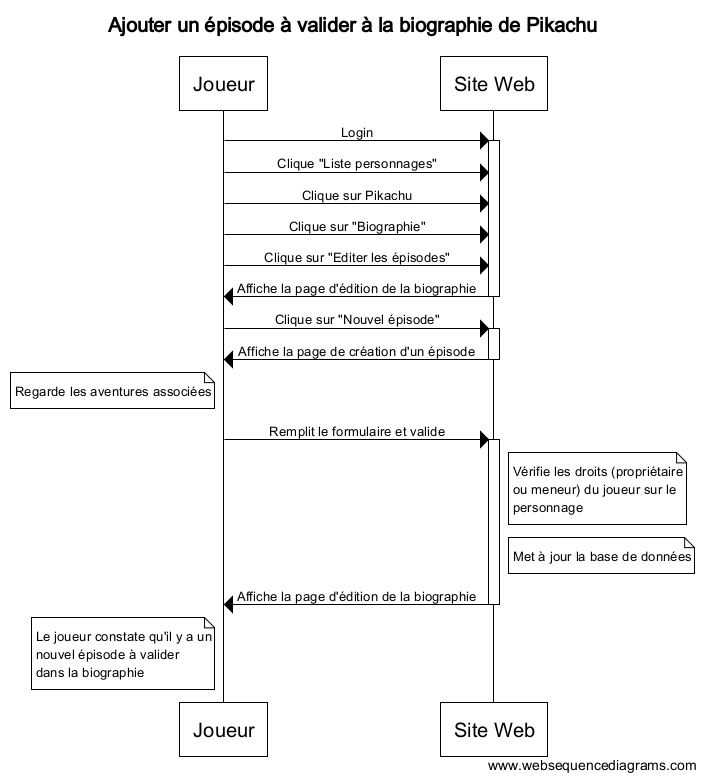
\includegraphics[scale=0.7]{sequence/AjouterEpisodeBiographie.png}
\end{center}

\subsubsection{Changer de meneur}

\begin{center}
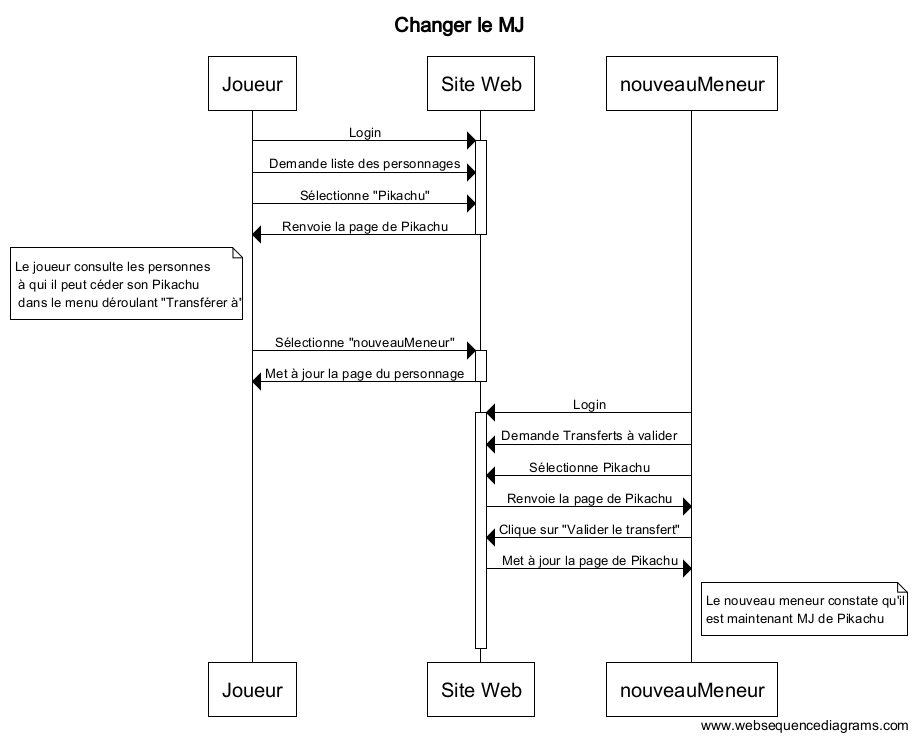
\includegraphics[scale=0.55]{sequence/ChangerleMJ.png}
\end{center}

\subsection{Diagramme de classes d'analyse}
Le sujet fournit une description des différents "objets" de l'application : partie, aventure, personnage, univers, biographie, épisode, paragraphe ...

Voici le diagramme de classes d'analyse que nous en avons tiré.

\textit{Nous avons considéré qu'une partie était simplement une aventure en cours (nous aurions pu faire de l'héritage mais l'avantage semblait mince par rapport aux inconvénients de la conversion d'une partie en aventure).\\
De même nous n'avons pas distingué les classes joueur et meneur de jeu : un joueur est meneur de jeu s'il est engagé dans les relations qui caractérisent un meneur de jeu (parties menés, personnages dont il est le meneur ...) Cela se justifie par le caractère dynamique de ce  statut : un joueur peut facilement devenir meneur de jeu ou arrêter de l'être, être un meneur de jeu semblait donc être plutôt une propriété dynamique des joueurs. }

% \begin{center}
\begin{figure}[ht!]
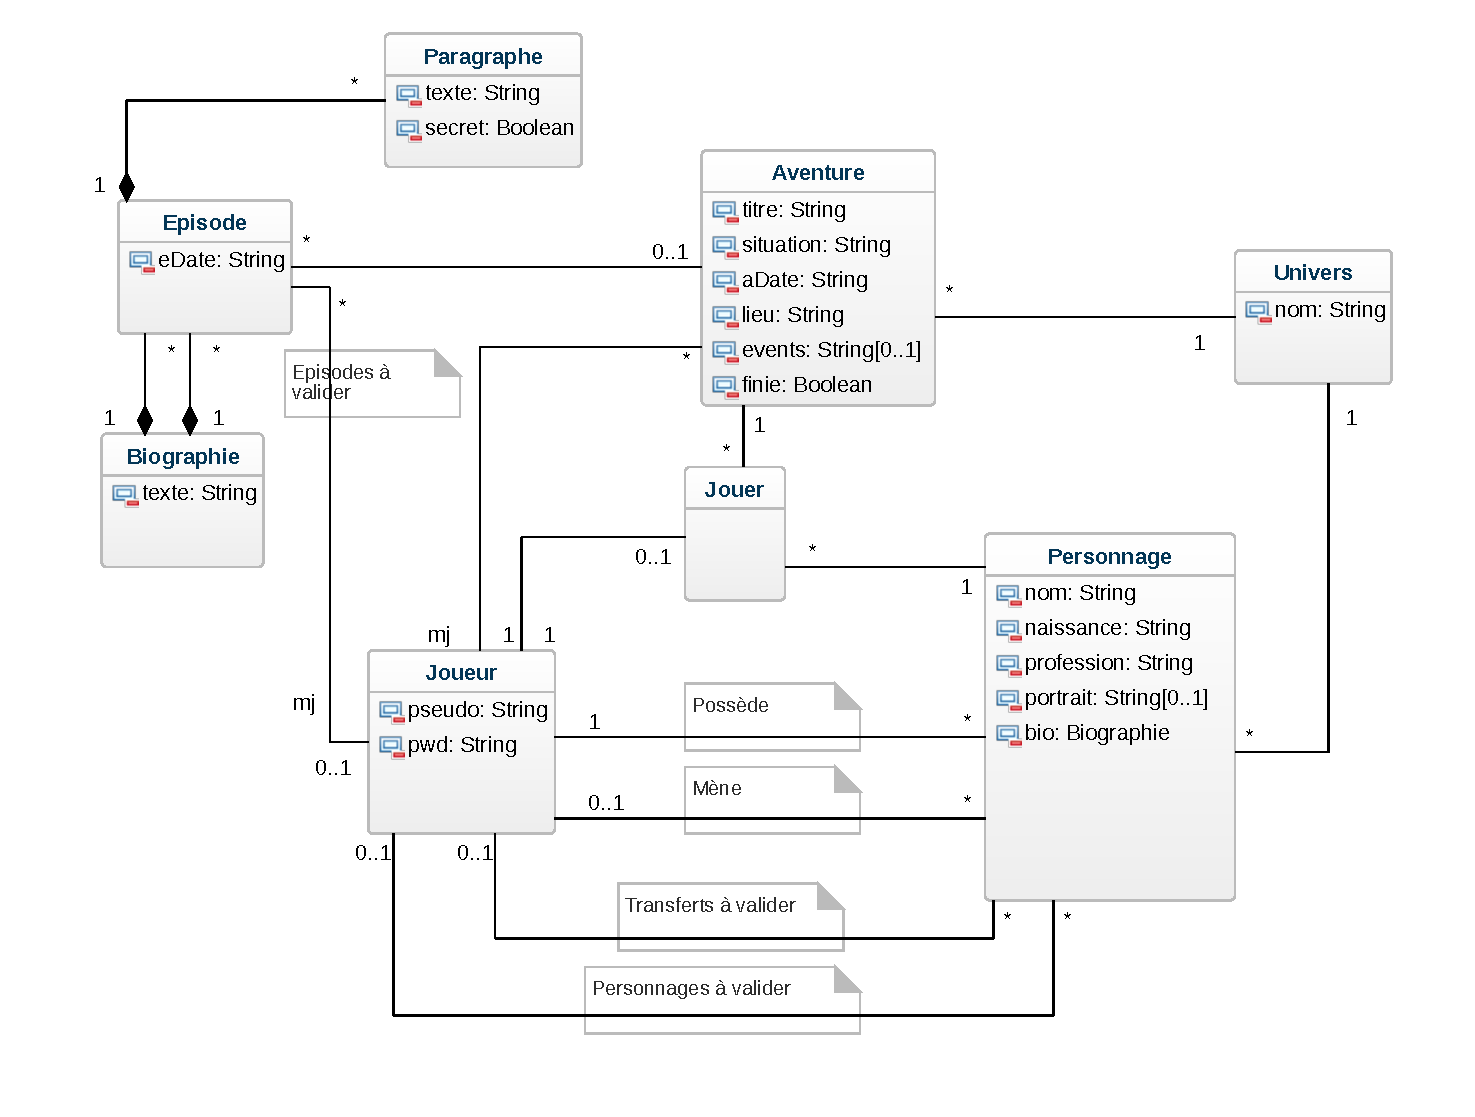
\includegraphics[scale=0.7]{analyse/classes.pdf}
\caption{Diagramme de classes d'analyse}
\end{figure}
% \end{center}







% (b) Document de conception :
% — L’architecture générale modèle-vue-contrôleur est imposée, mais indiquez comment vous la
% mettez en œuvre : quels sont les contrôleurs et les vues, comment tout s’articule-t-il.
% — Conception détaillée : diagramme de classes logicielles, diagrammes de séquence, diagrammes
% d’états-transitions si cela est pertinent. Ces diagrammes doivent être cohérents entre eux et
% avec l’implémentation. Il est inutile de fournir des diagrammes illisibles ou qui n’apportent
% aucune information ; il peut être en revanche utile d’ajouter un minimum de texte explicatif
% le cas échéant.

\newpage

\section {Conception}

\subsection {Architecture}

\subsubsection {Contrôleurs, Servlets}

Nous avons segmenté la gestion de l'application en différents Servlets contrôleurs :
\begin{itemize}
\item
\lstinline!AventureCtrl! : Servlet de gestion des différentes aventures

\item
\lstinline!BiographieCtrl! : Servlet de gestion des différentes biographies

\item
\lstinline!EpisodeCtrl! : Servlet de gestion des différents épisodes

\item
\lstinline!Main! : Contrôleur principal de l'application

\item
\lstinline!ParagrapheCtrl! : Servlet de gestion des différents paragraphes

\item
\lstinline!PersonnageCtrl! : Servlet de gestion des différents personnages
\end{itemize}


\subsubsection {Vue}

Les vues sont organisées en dossiers correspondant aux différents contrôleurs. Nous avons également tiré parti de l'héritage de vues JSP à l'aide de fichiers tag JSP (squelette principal contenu dans le fichier \lstinline!src/main/webapp/WEB-INF/tags/wrapper.tag!), et utilisé la librairie JSTL au sein des différentes vues.


\subsubsection {Modèle}

Nous avons modélisé chaque table relationnelle par une classe Java correspondante pour facilement gérer l'encapsulation en objets des différents éléments.


\subsubsection {DAO}

Pour les accès à la base de données, nous avons utilisé des DAO correspondant aux différentes classes du modèle ainsi que des classes abstraites correspondantes pour aider à la spécification originelle des différentes méthodes et faciliter la collaboration.



\subsection {Détail de la conception}

\subsubsection {Diagramme de classes final du modèle}

\begin{center}
% \begin{figure}[ht!]
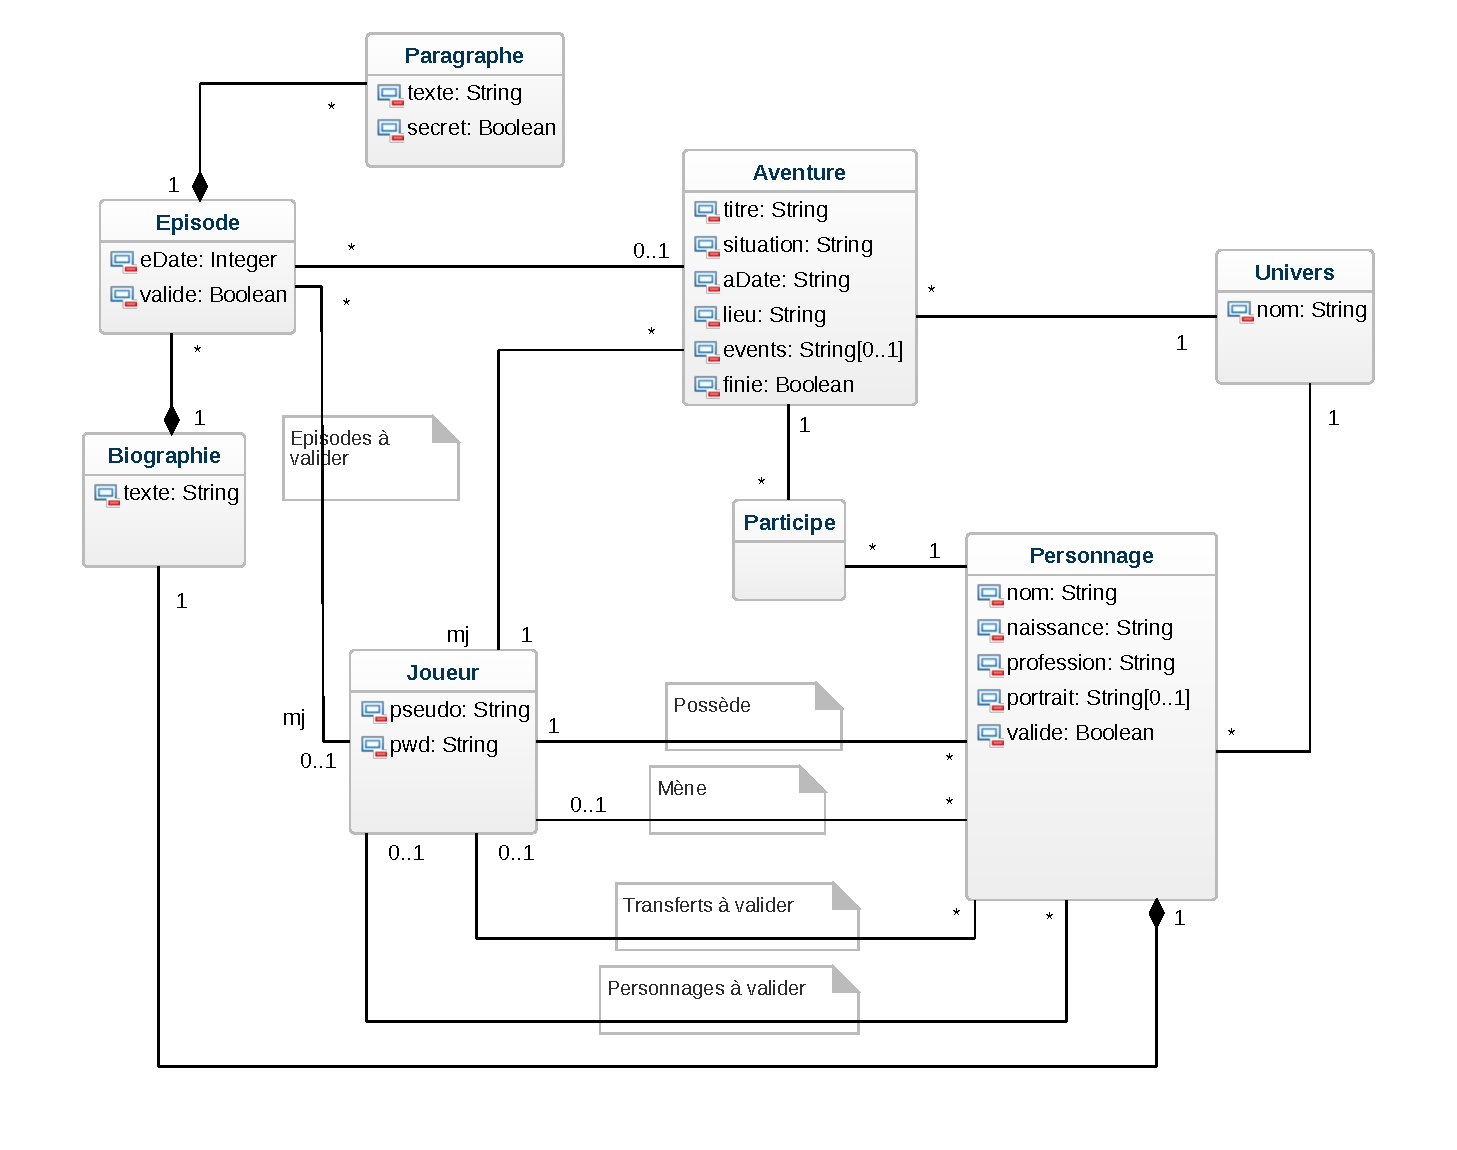
\includegraphics[scale=0.7]{conception/classes.pdf}
% \caption{Diagramme de classes du modèle}
% \end{figure}
\end{center}

L'implémentation Java correspondante comporte bien entendu des assesseurs pour permettre l'accès aux différents attributs privés.


\subsubsection {Diagramme de classes des DAO}

\begin{center}
% \begin{figure}[ht!]
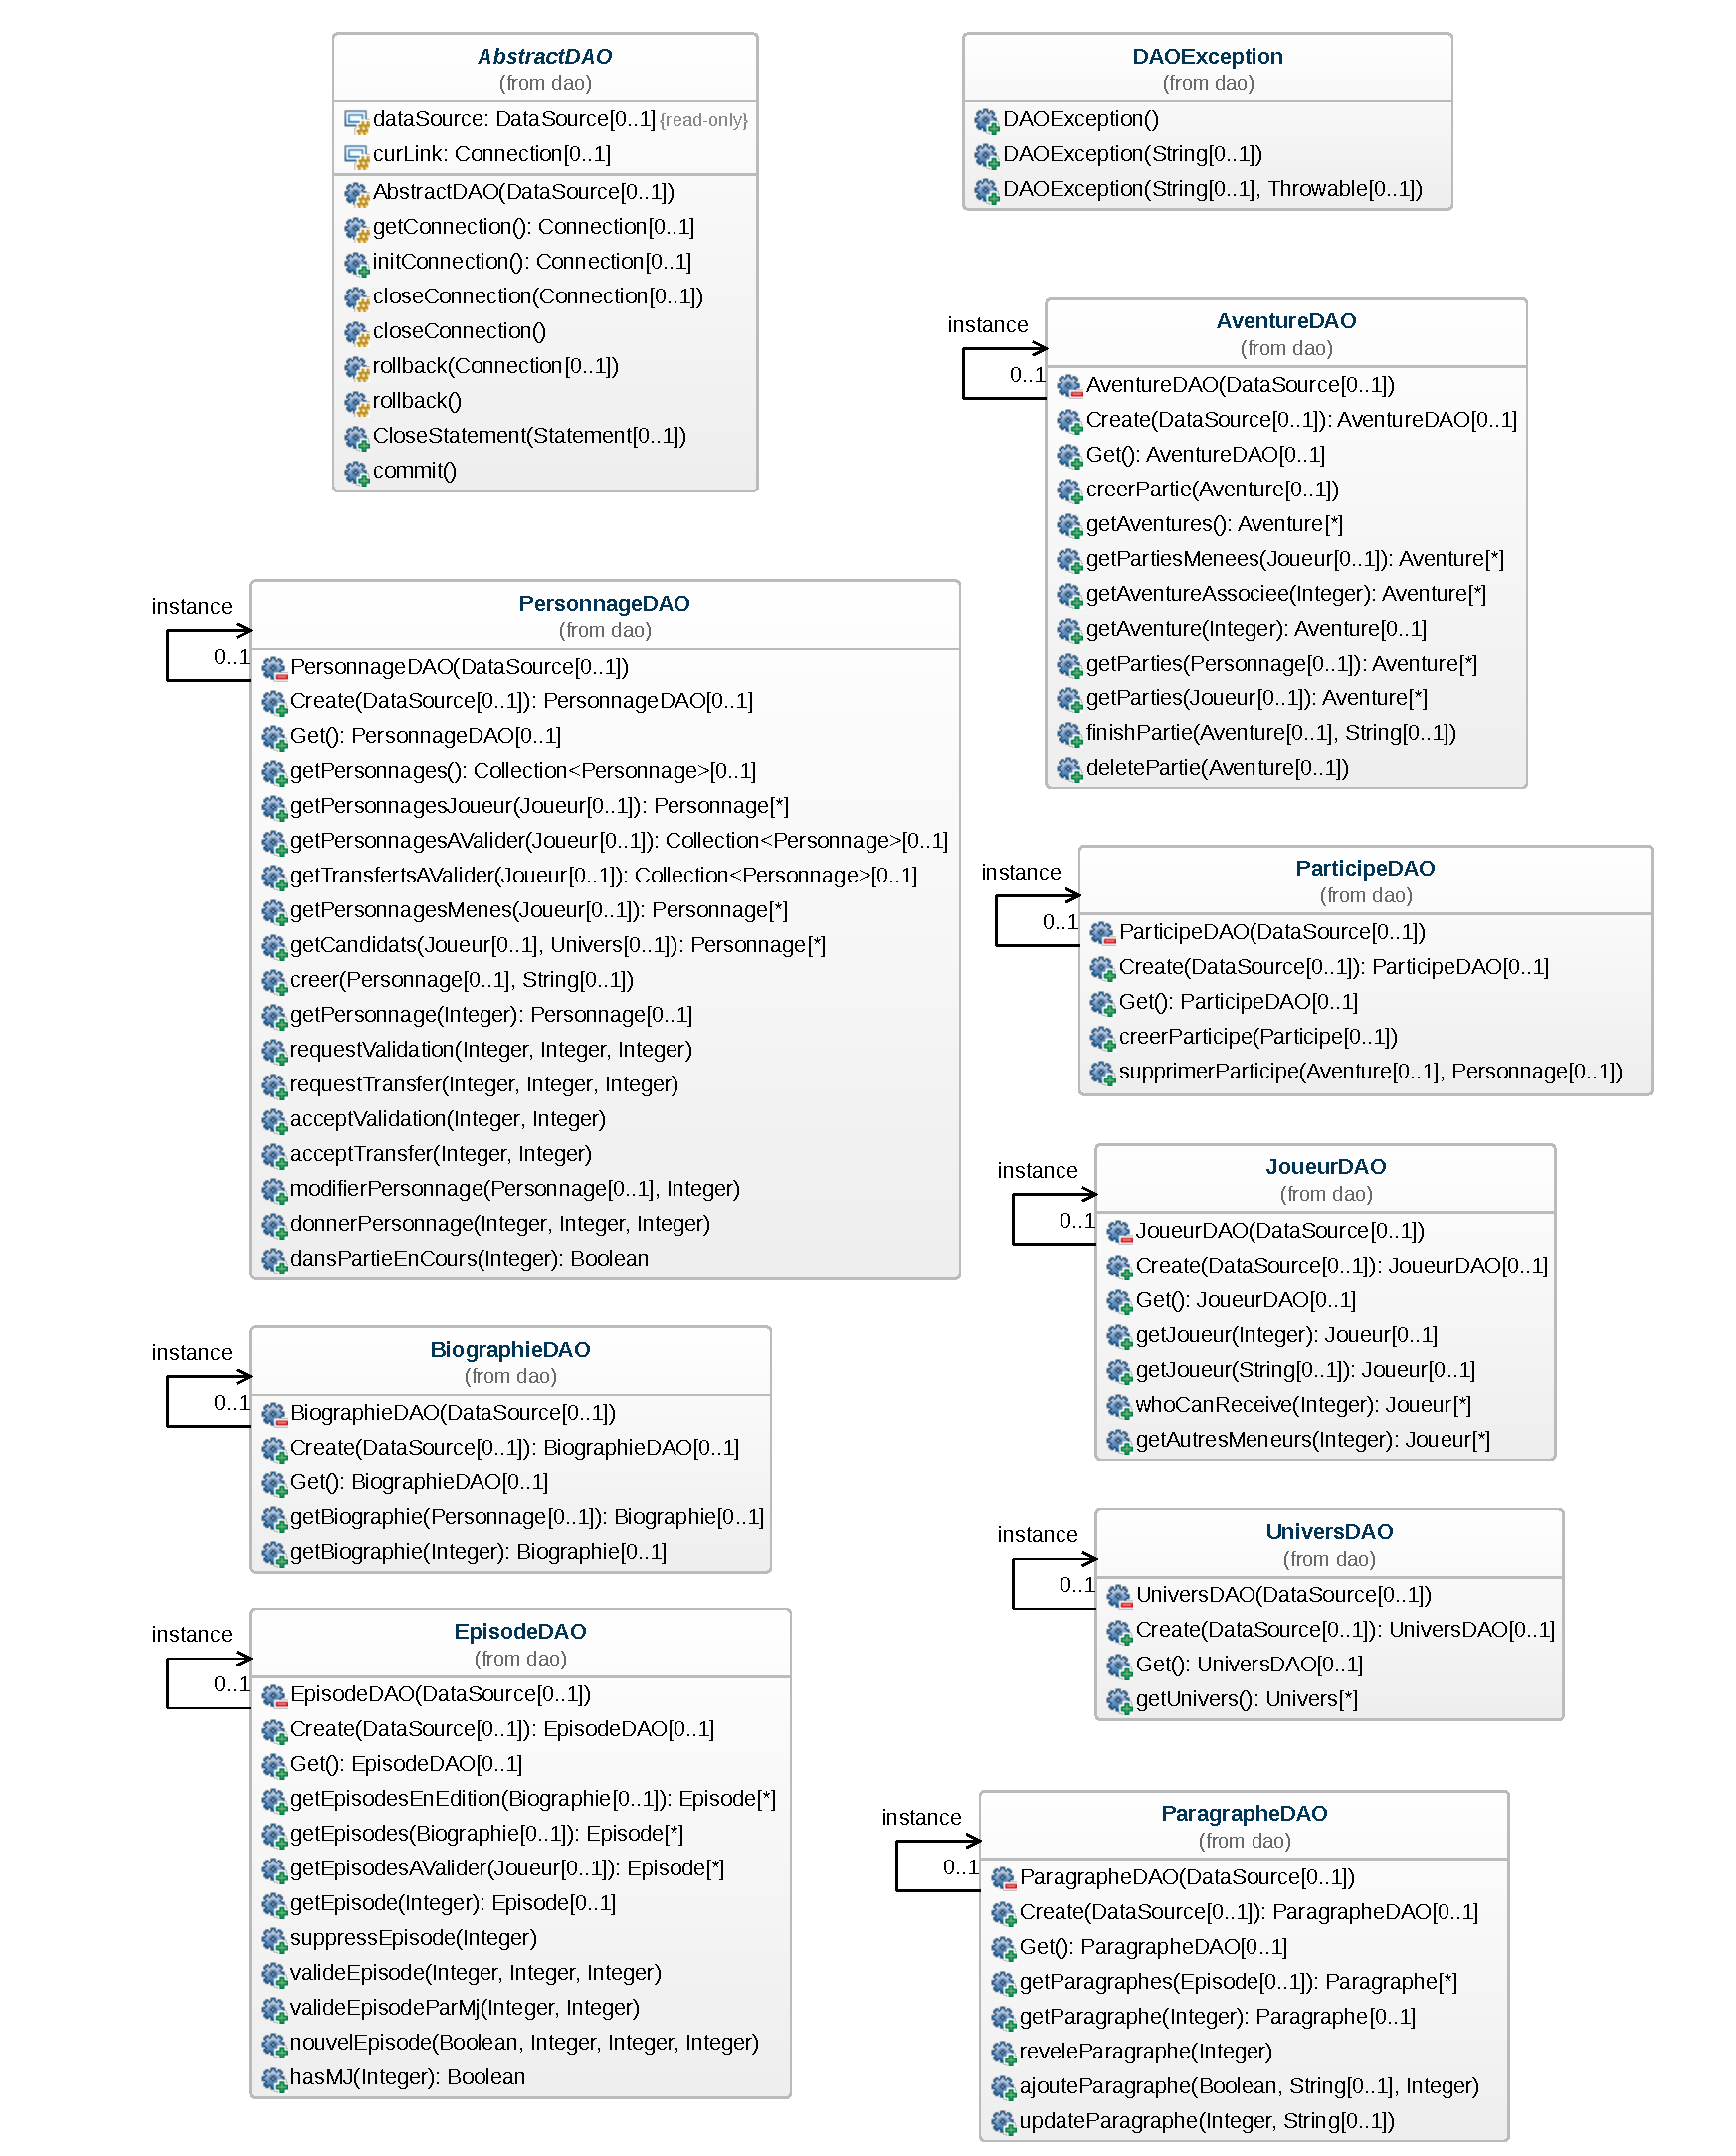
\includegraphics[scale=0.55]{conception/dao.pdf}
% \caption{Diagramme de classes du modèle}
% \end{figure}
\end{center}

Les différentes classes abstraites dont hérite chacun des singletons DAO ne sont pas représentées içi pour simplifier le diagramme. Elles héritent cependant bien toutes de \lstinline!AbstractDAO!.


\subsubsection {Diagramme de classes des contrôleurs}

\begin{center}
% \begin{figure}[ht!]
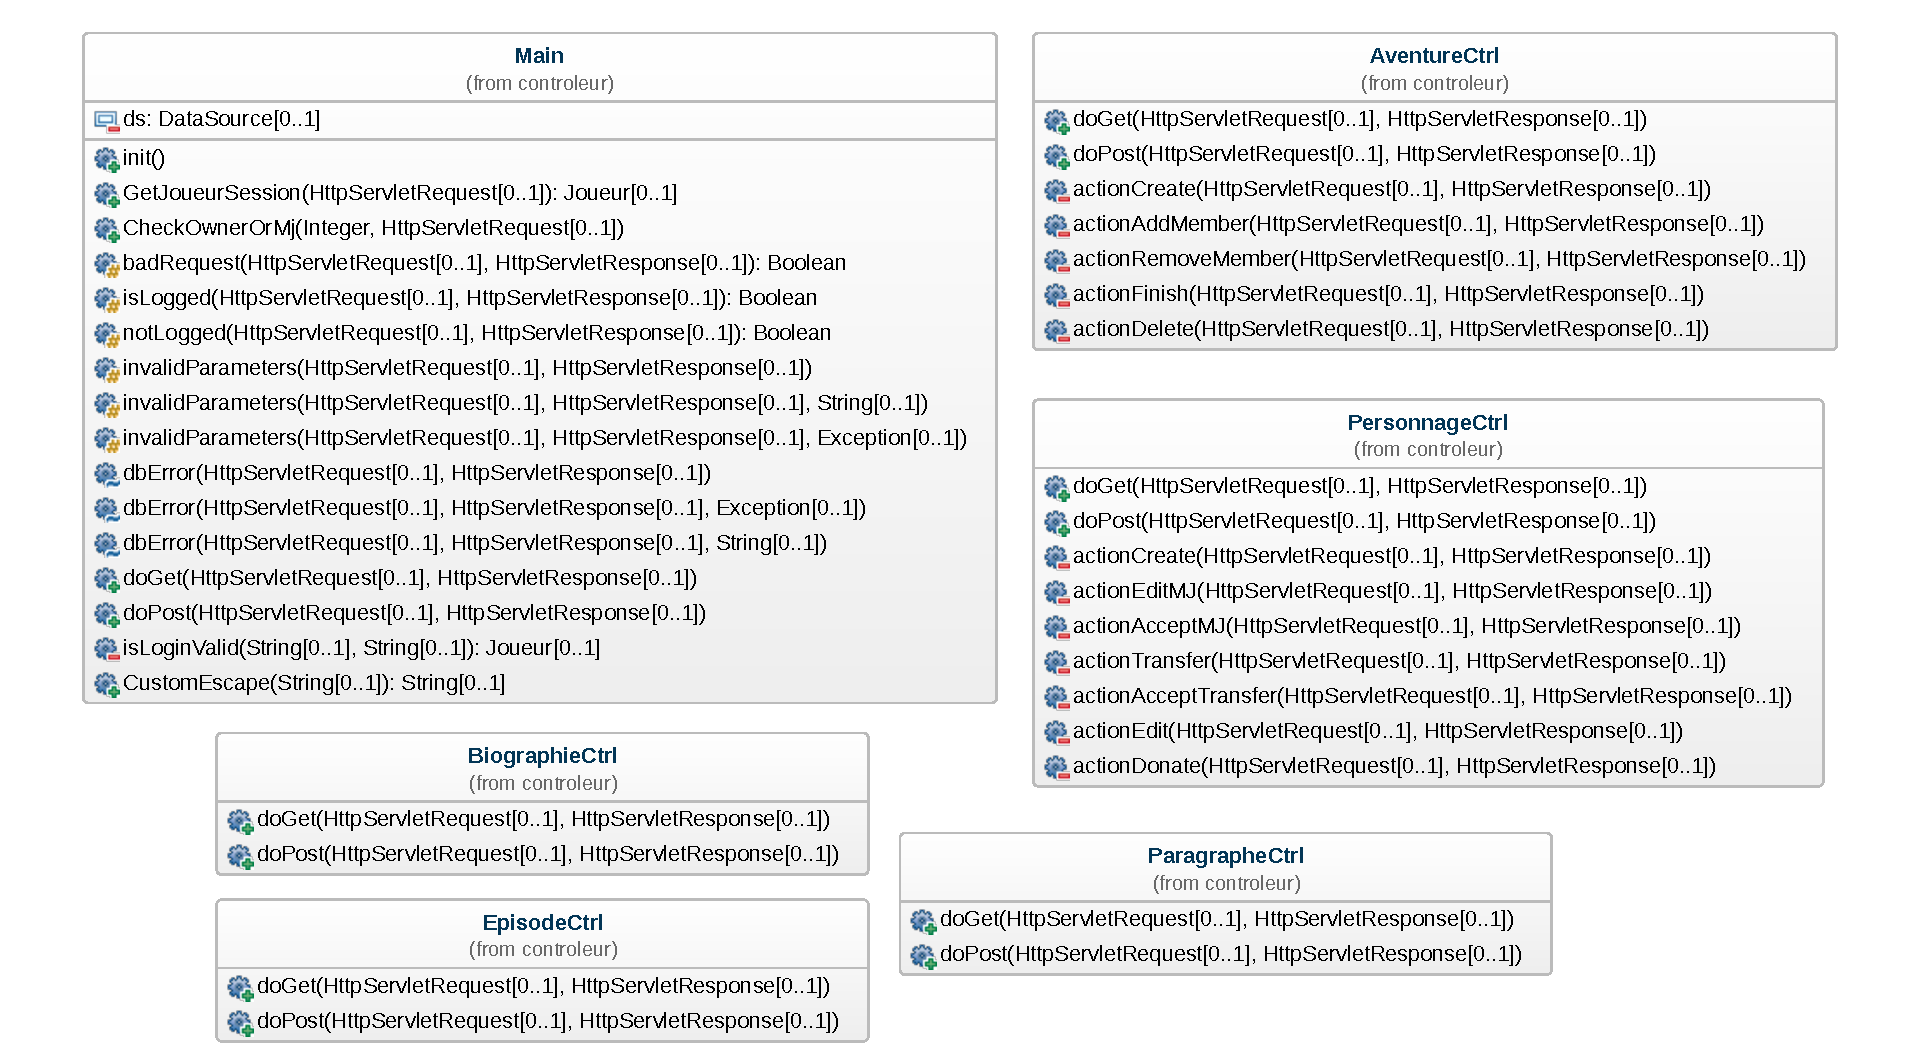
\includegraphics[scale=0.55]{conception/ctrl.pdf}
% \caption{Diagramme de classes du modèle}
% \end{figure}
\end{center}

On peut remarquer que les contrôleurs de biographies, d'épisodes et de paragraphes gèrent les différentes actions au sein de blocs switch et n'utilisent donc pas de méthodes secondaires spécifiques.


\subsubsection {Fonctionnement général de l'application}

L'application traite les requêtes au sein des contrôleurs correspondants, qui effectuent ensuite les appels DAO appropriés pour communiquer avec la base de données. La vue correspondante est alors affichée dans le cas d'une consultation de page, tandis qu'une redirection HTTP appropriée est effectuée lors de requêtes POST spécifiques (sauf en cas d'erreur, ou une page d'erreur descriptive est affichée).


\subsubsection {Diagrammes d'états-transitions pour la création d'épisodes, de personnages, ou de parties}

\begin{center}
% \begin{figure}[ht!]
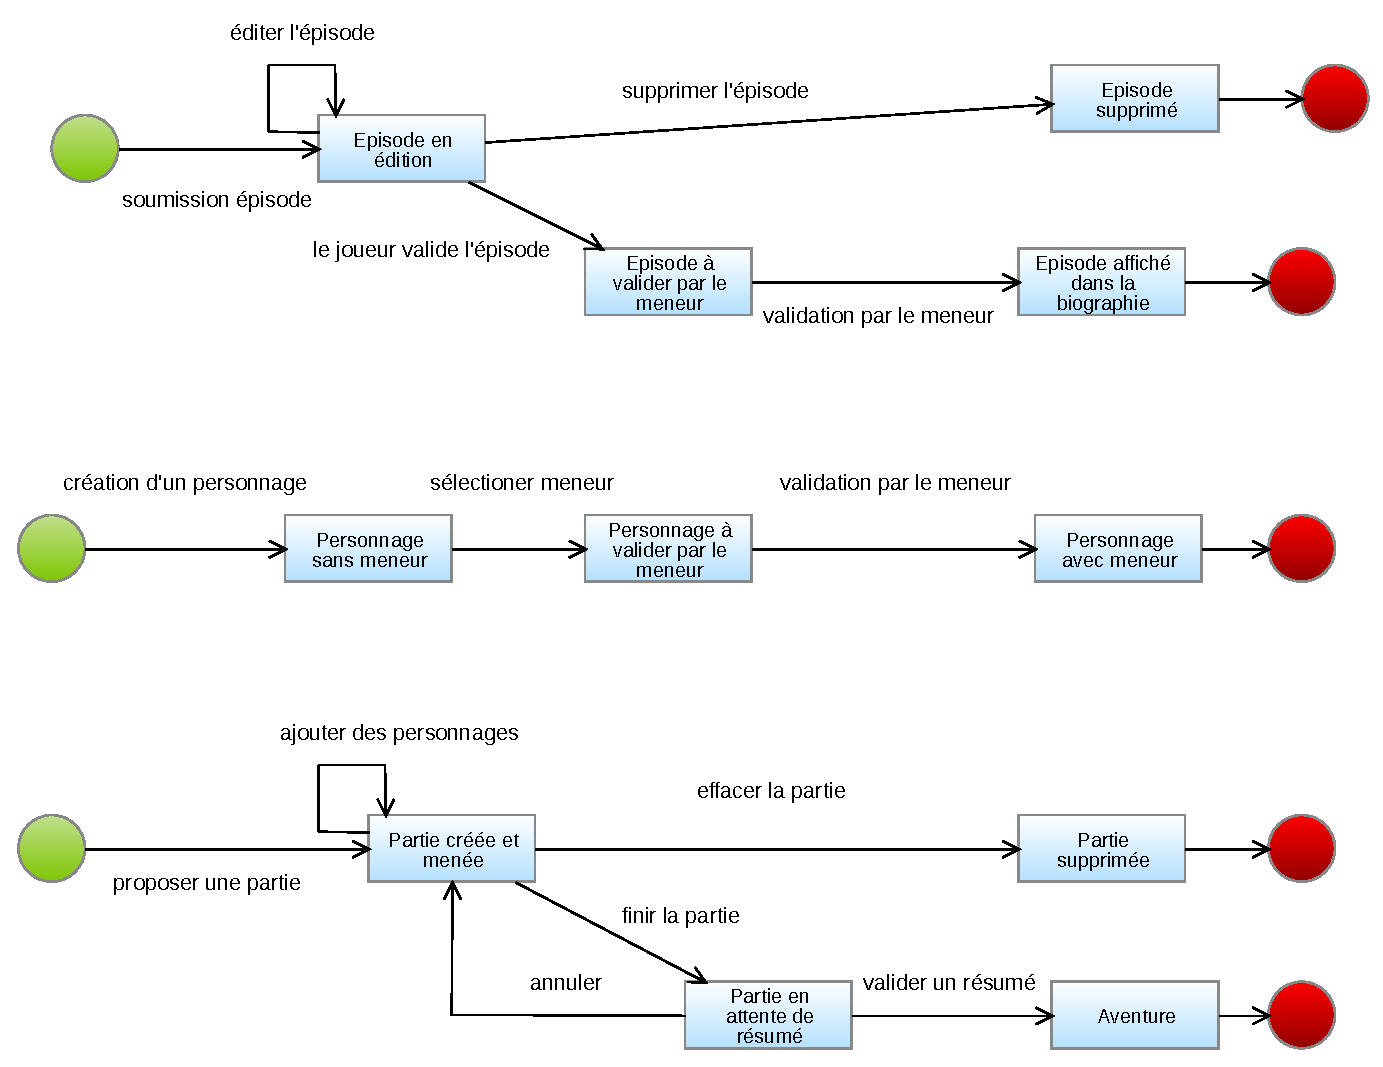
\includegraphics[scale=0.7]{conception/CreationEpisodesPersoParties.pdf}
% \caption{Diagrammes d'états-transitions pour la création d'épisodes, de personnages, ou de parties}
% \end{figure}
\end{center}

% \newpage
\subsection{Diagrammes de séquence}

\begin{center}
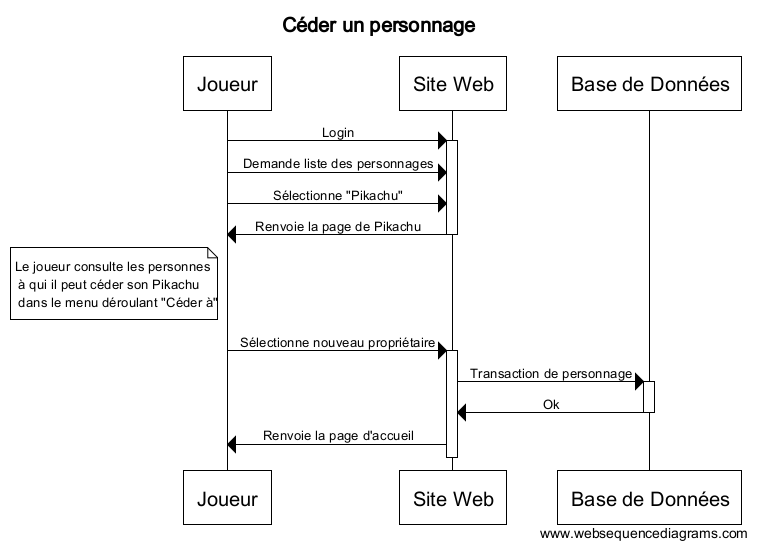
\includegraphics[scale=0.55]{sequence/CederUnPersonnage.png}
\end{center}

\begin{center}
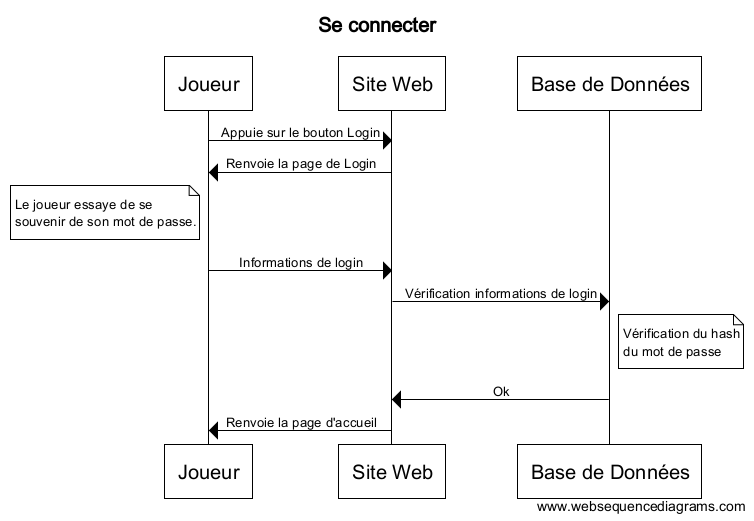
\includegraphics[scale=0.55]{sequence/Connexion.png}
\end{center}

\begin{center}
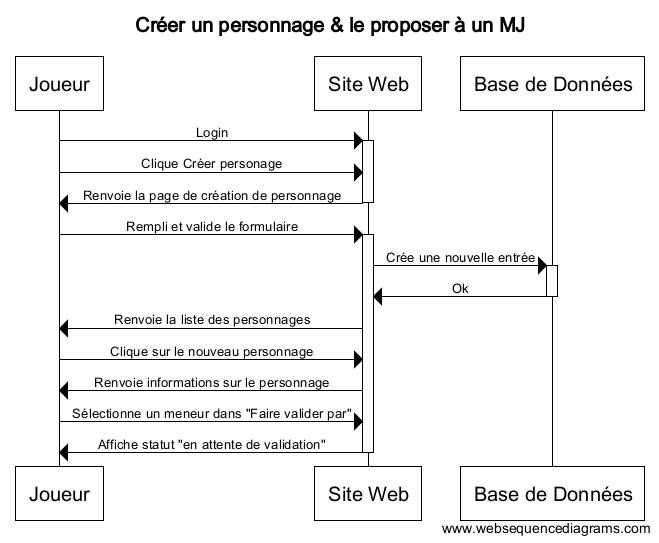
\includegraphics[scale=0.55]{sequence/CreerPersonnageEtProposerMJ.png}
\end{center}

\begin{center}
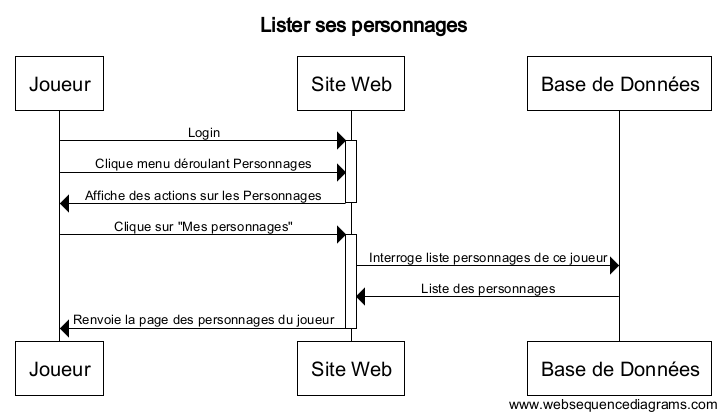
\includegraphics[scale=0.55]{sequence/ListerPersonnages.png}
\end{center}

\begin{center}
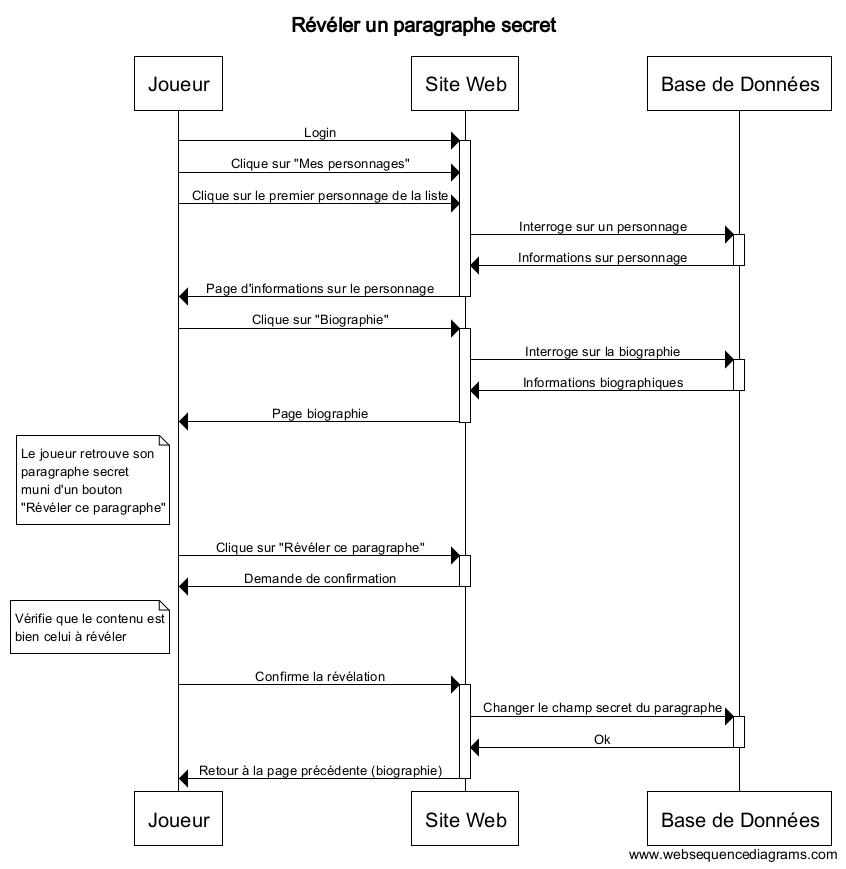
\includegraphics[scale=0.55]{sequence/RevelerParagraphe.png}
\end{center}

\begin{center}
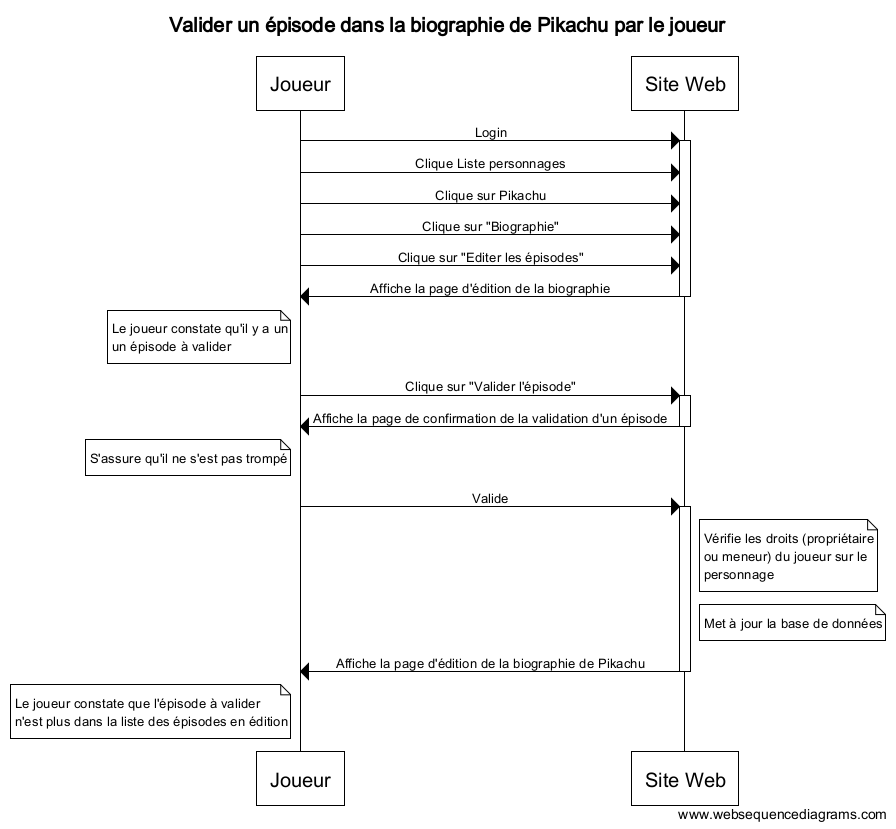
\includegraphics[scale=0.55]{sequence/ValiderEpisodeParJoueur.png}
\end{center}

\begin{center}
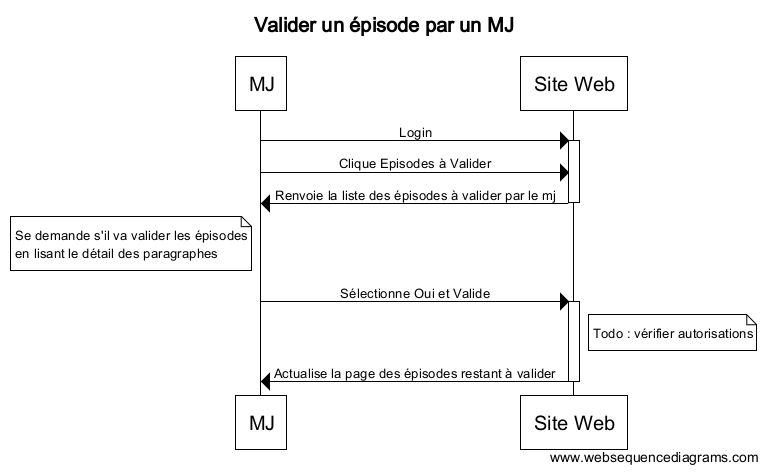
\includegraphics[scale=0.45]{sequence/ValiderEpisodeParMJ.png}
\end{center}


\section {Détails techniques}

L'application est normalement protégée contre tout type de faille XSS (via JSTL) et également des attaques par injection SQL. Les différents utilisateurs ne peuvent donc pas injecter de code HTML ou SQL lorsqu'ils ajoutent ou modifient des éléments au sein de l'application.

De plus la vérification des droits d'accès pour chaque type d'action a bien été implémentée, ainsi que la gestion des différentes erreurs dont le message reste intégré au design de l'application.

La gestion unicode des caractère a également été correctement gérée dans l'ensemble de l'application (aucun problème avec les accents par exemple).

Pour finir, les requêtes ont été écrites de manière à pouvoir assurer les accès concurrents (sérialisation des requêtes qui modifient la base de données), à l'aide de transactions (pas d'autocommit) et avec annulation des transactions en cas d'erreur.



\section {Manuel d'utilisation}

\subsection {Mise en route}

Différents joueurs sont installés dans la base d'origine.
Pour commencer, il suffit de se connecter avec les identifiants ci-dessous.

\subsubsection {Meneur admin}

Login : \lstinline!admin!, mot de passe : \lstinline!admin17Lord!


\subsubsection {Meneur Clara}

Login : \lstinline!Clara!, mot de passe : \lstinline!Vasto42!


\subsubsection {Joueur James}

Login : \lstinline!James!, mot de passe : \lstinline!james007tb!


\subsubsection {Meneur Max}

Login : \lstinline!Max!, mot de passe : \lstinline!max71Lord!




\subsection {Présentation générale}

L'application est composée d'une barre horizontale de navigation munie de différents sous-menus : Personnages, Parties et MJ.

Chacun d'entre-eux permet d'accéder à plusieurs liens correspondant, permettant l'accès aux différentes fonctionnalités de l'application.

Pour finir, chaque page est dotée d'un titre précis dans le navigateur, ce qui permet de bien distinguer chaque page dans son historique par exemple.

\subsection {Connexion / déconnexion}

Pour se connecter, il suffit de cliquer sur le bouton Login en haut à droite de la page d'accueil.

Une fois connecté, les différents sous-menus apparaissent. Un nouveau clic sur le bouton en haut à droite indiquant le nom d'utilisateur fait apparaitre un bouton Logout, qu'il suffit ensuite de cliquer pour se déconnecter.


\subsection {Les différents sous-menus}

\subsubsection {Personnages}

Ce menu permet d'accéder aux fonctionnalités suivantes :

\begin{itemize}
\item
Créer un personnage : Permet de créer un personnage

\item
Liste des personnages : Affiche la liste des personnages de l'application

\item
Mes personnages : Affiche la liste des personnages possédés

\end{itemize}


\subsubsection {Parties}

Ce menu permet d'accéder aux fonctionnalités suivantes :

\begin{itemize}
\item
Proposer une partie : Permet de créer une nouvelle partie

\item
Liste des parties : Affiche la liste des parties de l'application

\item
Mes parties : Affiche la liste des parties auxquelles a participé l'utilisateur, ainsi que le personnage utilisé

\end{itemize}

Le statut en cours ou terminée de chaque partie est également indiqué dans les différentes listes, d'ailleurs les aventures terminées sont même grisées.


\subsubsection {MJ}

\begin{itemize}
\item
Parties menées : Affiche la liste des parties menées

\item
Personnages menés : Affiche la liste des personnages menées

\item
Personnages à valider : Affiche la liste des personnages à valider

\item
Transferts à valider : Affiche la liste des personnages à transférer

\item
Episodes à valider : Affiche la liste des épisodes à valider

\end{itemize}


\subsection {Gestion des personnages}

\subsubsection {Créer un personnage}

Tout joueur a également la possibilité de créer un nouveau personnage, via le menu “Personnages” puis “Créer un personnage”. Il doit indiquer son univers, son nom, sa date de naissance, sa profession, et sa biographie initiale. Il a également la possibilité de donner un portrait au personnage via une url référencant une image.

Le joueur accède alors à la fiche du personnage. Il peut en demander la validation par un MJ en particulier.

\subsubsection {Consulter le détail d'un de ses personnages}

En cliquant sur l'un des personnages d'une liste, on arrive à sa page personnalle. Celle-ci permet de visualiser les différentes informations du personnage, en particulier : son nom, sa date de naissance, sa profession, son univers, son propriétaire, son meneur.
Il est également possible de modifier la profession, d'accéder à la biographie du personnage et à la liste des parties auxquelles il a participé.

Pour le propriétaire, il est aussi possible de faire valider / transférer le personnage s'il est invalide ou ne participe pas à une partie en cours, de même il possible de céder le personnage via une liste déroulante (sauf s'il participe à une partie en cours, car sinon des joueurs pourraient se retrouver avec plusieurs personnages dans une seule partie en cours).

C'est notamment sur cette même page que les meneurs de jeu peuvent accepter une demande de transfert ou de validation.


\subsubsection {Consulter et éditer la biographie d'un personnage}

La biographie est éditable si l'on est meneur ou propriétaire du personnage concerné.

Il suffit de cliquer sur les boutons "Nouvel épisode", "Nouveau paragraphe", et autres pour compléter, modifier ou valider des parties de la biographie.

Les différentes fonctionnalités suivantes sont disponibles :
\begin{itemize}
\item
Ajouter un nouvel épisode
\item
Supprimer un épisode non validé
\item
Demander la validation d'un épisode non validé
\item
Modifier un épisode non validé
\item
Ajouter un nouveau paragraphe à un épisode (choix de paragraphe secret ou non)
\item
Modifier un paragraphe existant
\end{itemize}

Un bouton révéler permet notamment de rendre les paragraphes secrets publics, avec une demande de confirmation dynamique et une implémentation {\sc ajax} de la fonctionnalité révéler.


\subsection {Gestion des parties}

\subsubsection {Proposer une partie}

Tout joueur a la possibilité de proposer une partie. Il doit indiquer : son univers, son titre, sa date, son lieu, ainsi que sa situation initiale. Il accède alors à la liste de ses parties menées, peut éditer sa nouvelle partie dont il devient le MJ, comme décrit dans la section précédente.

\subsubsection {Consulter le détail d'une partie}

En cliquant sur les parties d'une liste, on arrive à leur page personnalisée. Celle-ci permet de visualiser les différentes informations de la partie (nommée aventure si elle s'est terminée), en particulier : son nom, sa date, son lieu, son univers, sa situation initlale, son meneur. Il y est aussi possible d'accéder à la liste des participants (avec des boutons pour retirer des personnages si l'on en est le meneur).

Le meneur peut également ajouter des participants à l'aide d'une liste déroulante, terminer la partie en inscrivant un résumé des événements dans la fenêtre dynamique qui apparaît, ou encore la supprimer si elle n'est pas encore finie (avec demande de confirmation dynamique).


\subsection {Tâches de MJ}

\subsubsection {Accéder à la liste de ses parties menées}

Via le menu “MJ”, puis “Parties menées”. Le joueur obtient alors la liste des parties dans lesquelles il est meneur de jeu. Les fonctionnalités d’une telle liste sont décrites ci-dessus.

\subsubsection {Accéder à la liste de ses personnages menés}

Via le menu “MJ”, puis “Personnages menés”. Le joueur obtient alors la liste des personnages dont il est le meneur. Les fonctionnalités d’une telle liste sont décrites ci-dessus.

\subsubsection {Accéder à la liste de ses personnages à valider}

Via le menu “MJ”, puis “Personnages à valider”. Le joueur obtient alors la liste des personnages pour lesquels un autre joueur à demandé une validation. Le MJ peut alors consulter la fiche descriptive du personnage puis s’il le désire, le valider.

\subsubsection {Accéder à la liste de ses transferts à valider}

Via le menu “MJ”, puis “Transferts à valider”. Le joueur obtient alors la liste des transferts pour lesquels un autre joueur à demandé à ce que le MJ d’un de ses personnages soit le joueur courant. Ce dernier peut alors consulter la fiche descriptive du personnage puis s’il le désire, valider le transfert. Il n’est pas MJ du personnage tant qu’il n’a pas fait cette validation.

\subsubsection {Accéder à la liste de ses épisodes à valider}

Via le menu “MJ”, puis “Episodes à valider”. Lorsqu'un joueur veut ajouter un épisode à la biographie de son personnage, l’épisode doit être validé par le MJ. C’est le but de cette section de permettre au MJ de consulter la liste des épisodes ajoutés dont la validation a été demandée par le joueur, puis s’il le souhaite d’effectuer cette validation.



% (d) Bilan sur les outils de modélisation utilisés, en particulier les problèmes rencontrés, ainsi que
% les solutions trouvées. Il vous est demandé dans cette partie de bien préciser les logiciels, en particulier les modeleurs UML que vous avez utilisés.

\section {Bilan sur les outils de modélisation utilisés}

Au cours de ce projet nous avons utilisé différents outils de modélisation.

Au niveau des modeleurs UML, il n'est pas évident de trouver des outils gratuits de bonne qualité, et nous avons finalement choisi d'utiliser l'outil GenMyModel qui permet une modélisation simple et collaborative. Un autre outil de relativement bonne qualité aurait pu être PlantUML, mais il a le désavantage de ne pas être entièrement graphique (moins facile à utiliser). Nous avons également testé ArgoUML, mais ce logiciel n'était pas de très bonne qualité.

Certains diagrammes ont également été réalisés à l'aide de Visual Studio (diagramme des cas d'utilisation), ou encore de Web Sequence Diagrams (diagrammes de séquence, pas d'export vectoriel sans premium).


\end{document}


